\documentclass{article}

% if you need to pass options to natbib, use, e.g.:
% \PassOptionsToPackage{numbers, compress}{natbib}
% before loading nips_2017
%
% to avoid loading the natbib package, add option nonatbib:
% \usepackage[nonatbib]{nips_2017}

\usepackage[final]{nips_2017}

% to compile a camera-ready version, add the [final] option, e.g.:
% \usepackage[final]{nips_2017}

\usepackage[utf8]{inputenc} % allow utf-8 input
\usepackage[T1]{fontenc}    % use 8-bit T1 fonts
\usepackage{hyperref}       % hyperlinks
\usepackage{url}            % simple URL typesetting
\usepackage{booktabs}       % professional-quality tables
\usepackage{amsfonts}       % blackboard math symbols
\usepackage{nicefrac}       % compact symbols for 1/2, etc.
\usepackage{microtype}      % microtypography
\usepackage{graphicx}
\usepackage{amsmath}


\title{CS5785 Final Exam Report on Build a Large-scale Image Search Engine}

% The \author macro works with any number of authors. There are two
% commands used to separate the names and addresses of multiple
% authors: \And and \AND.
%
% Using \And between authors leaves it to LaTeX to determine where to
% break the lines. Using \AND forces a line break at that point. So,
% if LaTeX puts 3 of 4 authors names on the first line, and the last
% on the second line, try using \AND instead of \And before the third
% author name.

\author{
%   David S.~Hippocampus\thanks{Use footnote for providing further
%     information about author (webpage, alternative
%     address)---\emph{not} for acknowledging funding agencies.} \\
%   Department of Computer Science\\
%   Cranberry-Lemon University\\
%   Pittsburgh, PA 15213 \\
%   \texttt{hippo@cs.cranberry-lemon.edu} \\
  %% examples of more authors
  %% \And
  %% Coauthor \\
  %% Affiliation \\
  %% Address \\
  %% \texttt{email} \\
  %% \AND
  %% Coauthor \\
  %% Affiliation \\
  %% Address \\
  %% \texttt{email} \\
  %% \And
  %% Coauthor \\
  %% Affiliation \\
  %% Address \\
  %% \texttt{email} \\
  %% \And
  %% Coauthor \\
  %% Affiliation \\
  %% Address \\
  %% \texttt{email} \\
}

\begin{document}
% \nipsfinalcopy is no longer used

\maketitle

\begin{abstract}
  
  We are challenged to predict relevance images given the description. We have designed and experimented with 3 text-based methods to complete the task. This paper will introduce the  BOW+KNN, maolixuan model, baihuajun model. We have found the different weight for connection between the image feature and that between text descriptions, and the best performing method is image-to-description method with an accuracy score of 0.3695 on Kaggle.
\end{abstract}

\section{Introduction}

This competition challenges us to retrieve target image from natural language descriptions in sentences. We are given a testing image set and train image set, the convolutional and classificational feature vectors for each image, sentence descriptions for training images, and textual tags for both training and testing images.

Text-based image retrieval is in terms of how users make queries to the image database, and in which form the images information is stored.

In Text-based image retrieval, images are annotated with a textual description (Tags) and their retrieval is based on matching the user’s textual query (Descriptions) to the annotation of the image.Text-based image retrieval requires considerable amounts of pre-annotated tags or captions of images, which is hard to obtain. In this paper we present a series of different approaches of image retrieval using a combined methods of Text-based image retrieval and Content-based image retrieval techniques.

\section{Related Work}

\section{Model Architecture}

\subsection{Bag of Word(BoW) Representation }
\subsubsection{Word Dictionary}

First, we design a function to generate the word dictionary that is used in the calculation of BoW. By leveraging \emph{Natural Language Toolkit(NLTK)}, we can analyze each description sentence in the training set and find out what role each word plays in the sentence. Intuitively, noun, adjective and verb are the most informative parts in a sentence, which are the greatest help for one trying to connect pictures with a sentence. However, preposition like 'in', 'with', etc. and article like 'the' and 'a' reveal little information about what picture this sentence tries to describe. This is why we decide to only extract noun, adjective and verb from description sentences and make them potential candidates of the word dictionary.

In addition, when we skim through all those candidates, we find some words are really uncommon and rarely used, which leads us to apply an occurrence time threshold $t$ so that only words that appear more that $t$ times can be a valid candidate.\footnote{we use $t=15$ and $t=20$ during the whole process}

Finally, we generated multiple versions of word dictionaries for training different models so that we may assemble them to generate robuster and more powerful models. We generate three versions of word dictionaries that consist of noun, noun\&adjective, noun\&adjective\&verb respectively.
\begin{figure}[h]
  \centering
  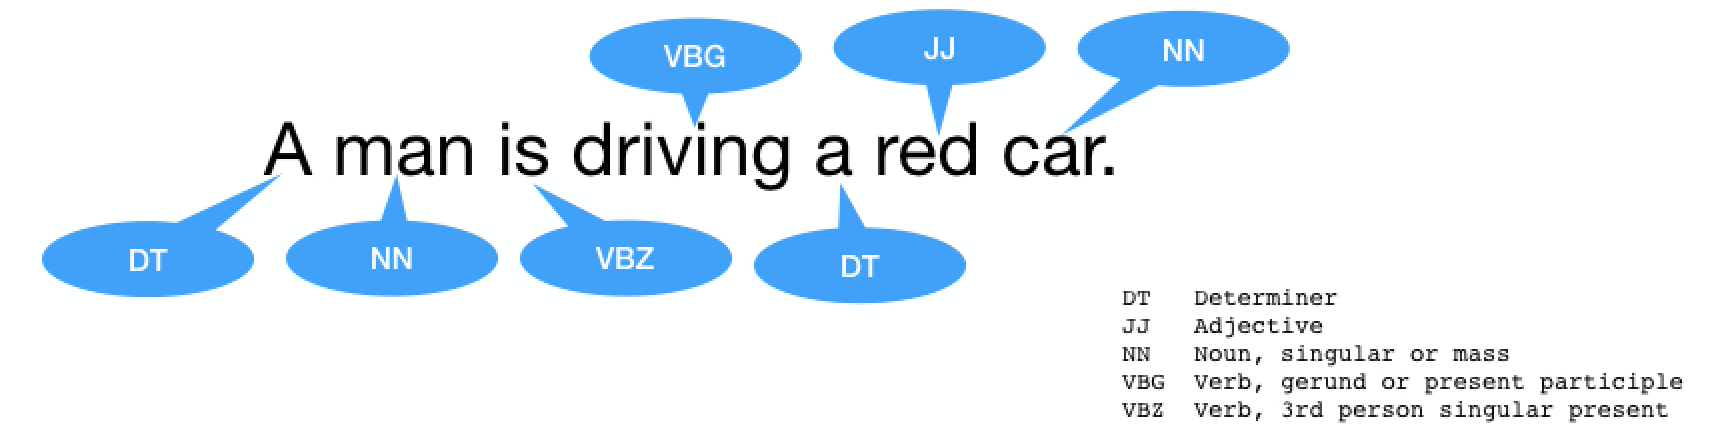
\includegraphics[width=\textwidth]{SentenceAnalysis}
  \caption{Sentence Analysis Example}
\end{figure}

\subsubsection{BoW Vector}

For each image's descriptions in the training and testing set, we can generate BoW vectors based on different versions of dictionaries. We call them \textbf{BoW train} and \textbf{BoW test}.

\subsection{Neural Network}

In this section, we try to build Neural Network(NN) models that map BoW representation space onto image feature space.

We use noun\&adjective dictionary to generate BoW representation for both training and testing descriptions, which would be used as model input during the training.

And then we build two NN models that regress 2048-dimensional \emph{resnet1000intermediate} and 1024-dimensional \emph{resnet1000}.

Two NN models have similar architecture:

\begin{description}
  \item[$\bullet$ Layer] One input layer (1000 neurons), One output layer(1000 neurons), Two hidden layers(2000 neurons each)
\end{description}
\begin{description}
  \item[$\bullet$ Activation] ReLu
\end{description}
\begin{description}
  \item[$\bullet$ Layer Type] Fully Connected
\end{description}
\begin{description}
  \item[$\bullet$ Dropout] Each Layer(except output layer) is followed by a Dropout layer with the 0.1 dropout rate.
\end{description}

Firgure2 demonstrates the architecture visually. 
\begin{figure}[h]
  \centering
  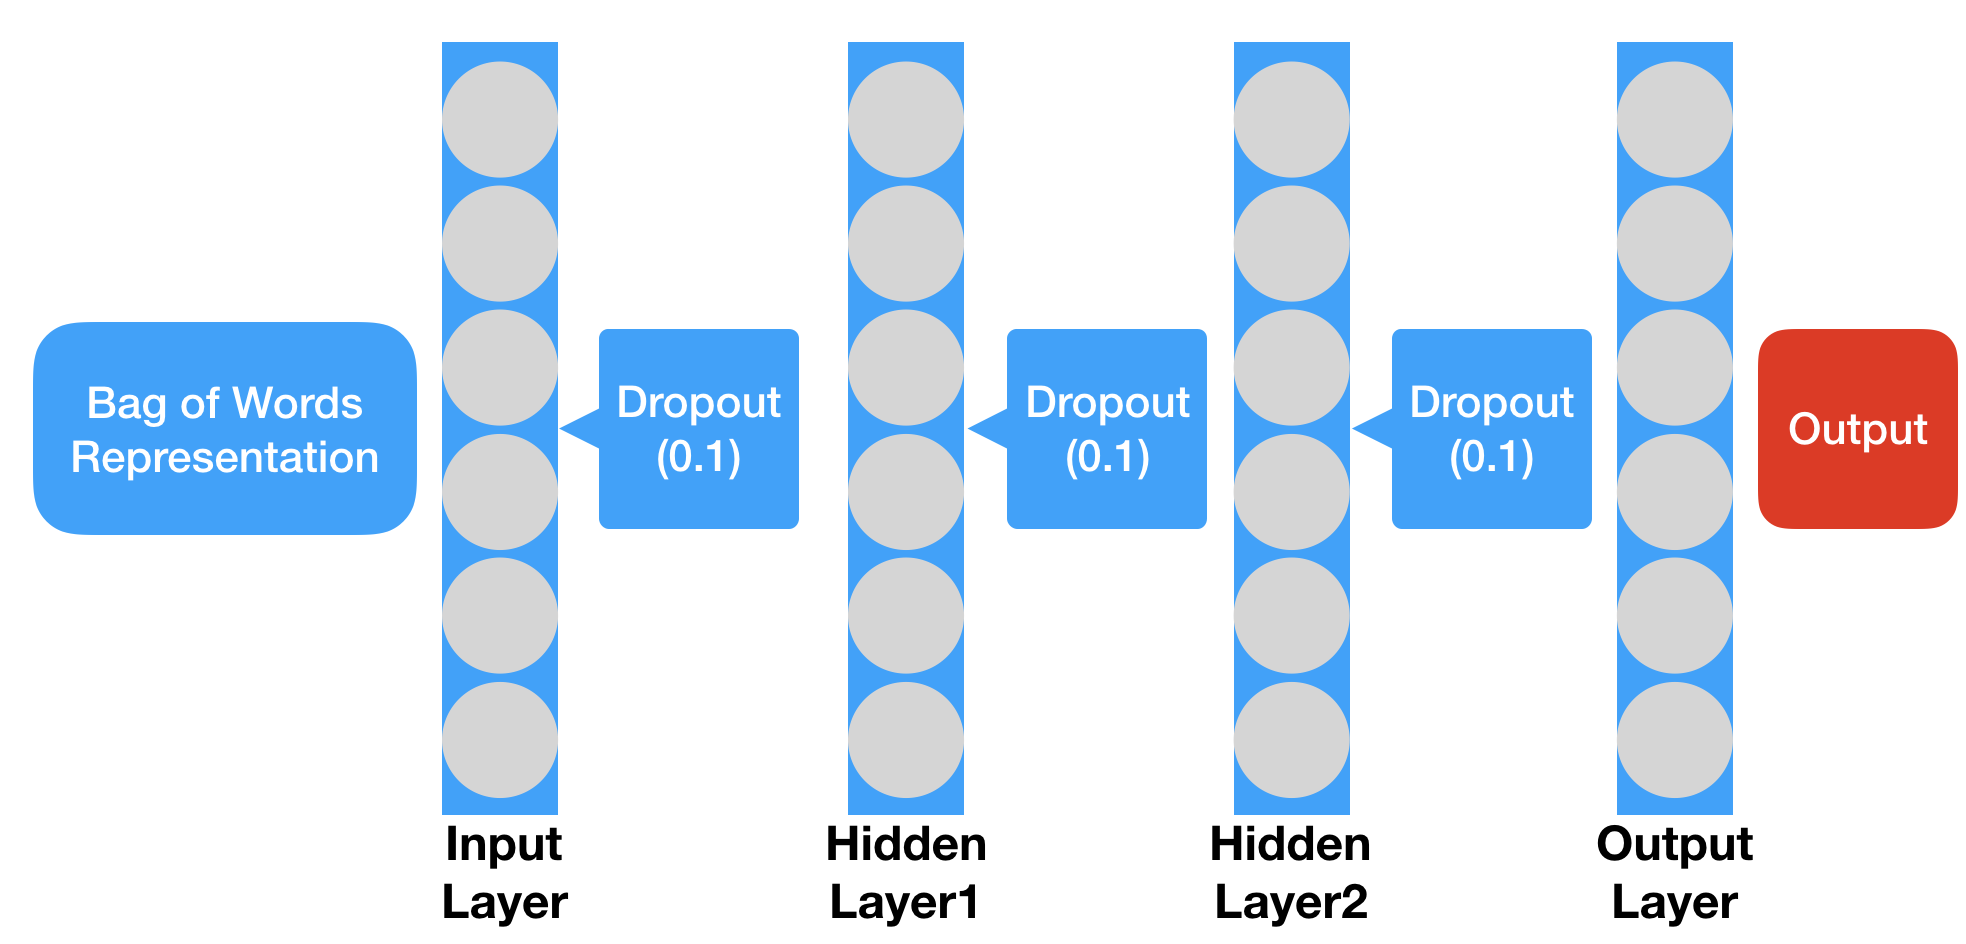
\includegraphics[width=\textwidth]{NeuralNetworkArchitecture}
  \caption{Neural Network Architecture}
\end{figure}

\subsection{Partial Least Square Regression}

After trying the first type of model, we start to think that by interpreting the data of image features, we could be able to calculate the semantic representation of the images. So it is worth trying to build a model that connect the image features with its BoW representation.

After some literature review, we find that Partial Least Square Regression(PLSR) could be a good way of building a model between one source of data and another. 

We build PLSR models to map image feature space to BoW representation space so that for each image, we can know what description it fits into most. So for each description in the test set, we compare its BoW with the predicted BoWs of the images in the test set and fetch the most similar 20 images.

In the end, we trained 3 different PLSR models, each of which tries to extract different information from the image features so that they could be useful to build a robust ensemble model.
\begin{equation*}
\begin{aligned}
& 1000D\;Feature \rightarrow PLSR(n\_component = 400) \rightarrow BoW_{noun\_adj\_verb\_dict} \\
& 2048D\;Feature \rightarrow PLSR(n\_component = 400) \rightarrow BoW_{noun\_adj\_dict}  \\
& 2048D\;Feature \rightarrow PLSR(n\_component = 500) \rightarrow BoW_{noun\_adj\_verb\_dict}
\end{aligned}
\end{equation*}

\begin{figure}[h]
  \centering
  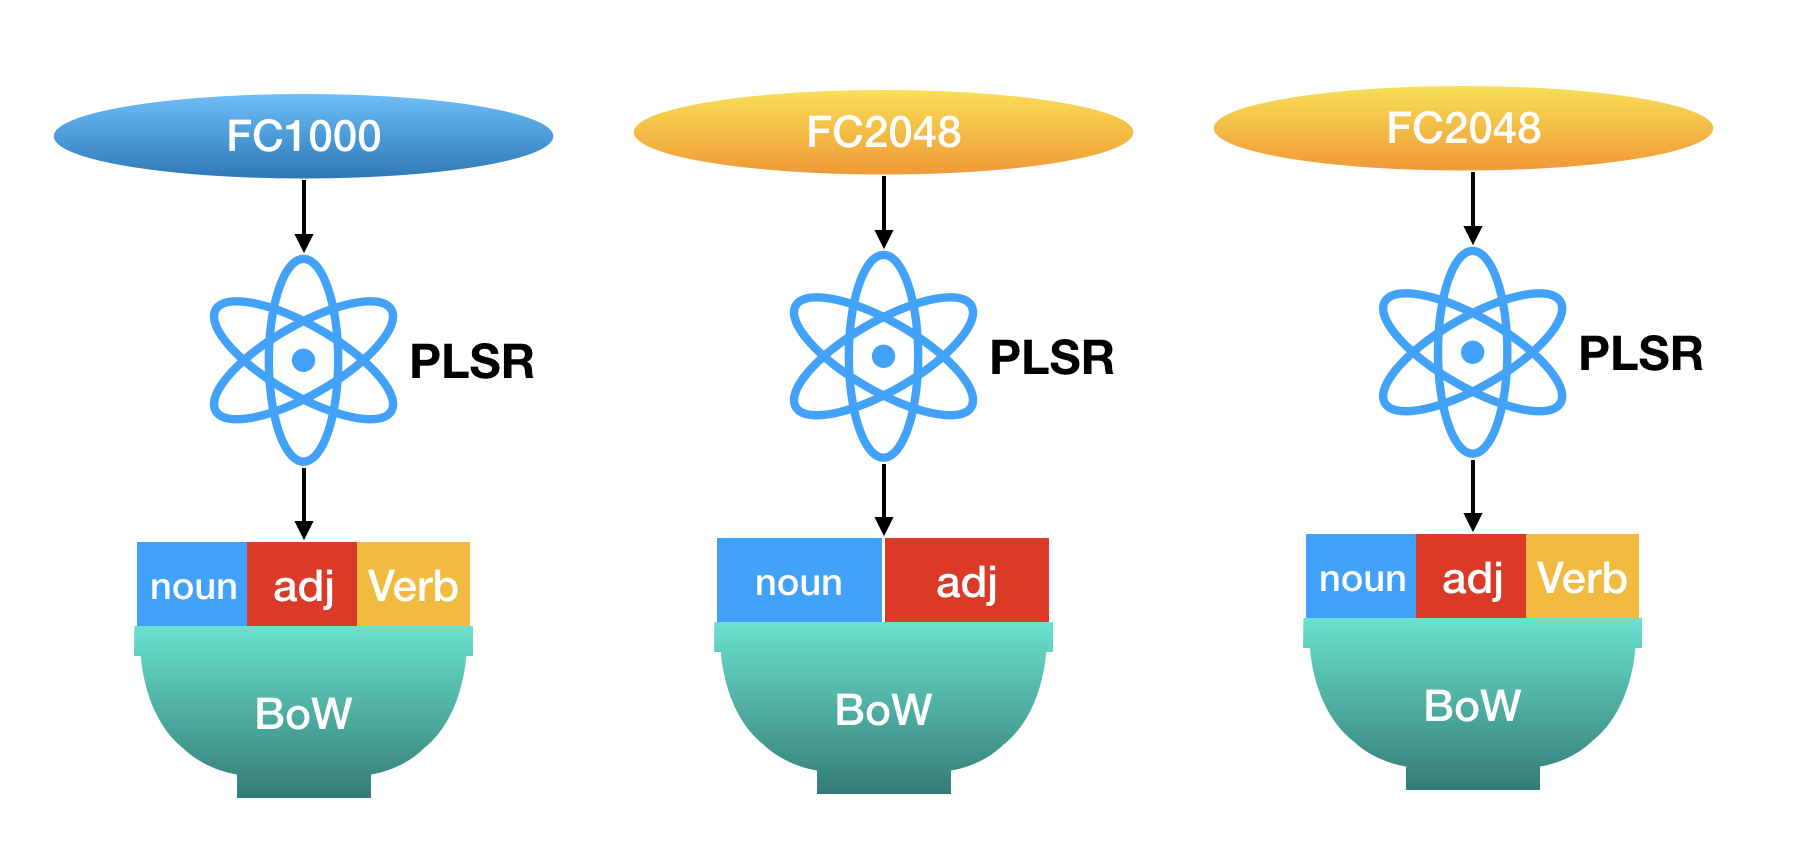
\includegraphics[width=\textwidth]{PLSR_models}
  \caption{Partial Least Square Regression Models Overview}
\end{figure}

\subsection{Similarity Evaluation}
\subsubsection{Neural Network Model}

NN models map BoW representation to image features. In the testing phase, we map the BoW vector of each set of descriptions to a 1000-dimensional feature vector and a 2048-dimensional feature vector. Then calculate the cosine distance between these two vectors and the feature vectors of the images in the testing set, which give us a quantitative measurement of how well the images match the descriptions. We can pick the 20 images with the smallest cosine distance as the image retrieval result. 

\begin{figure}[h]
  \centering
  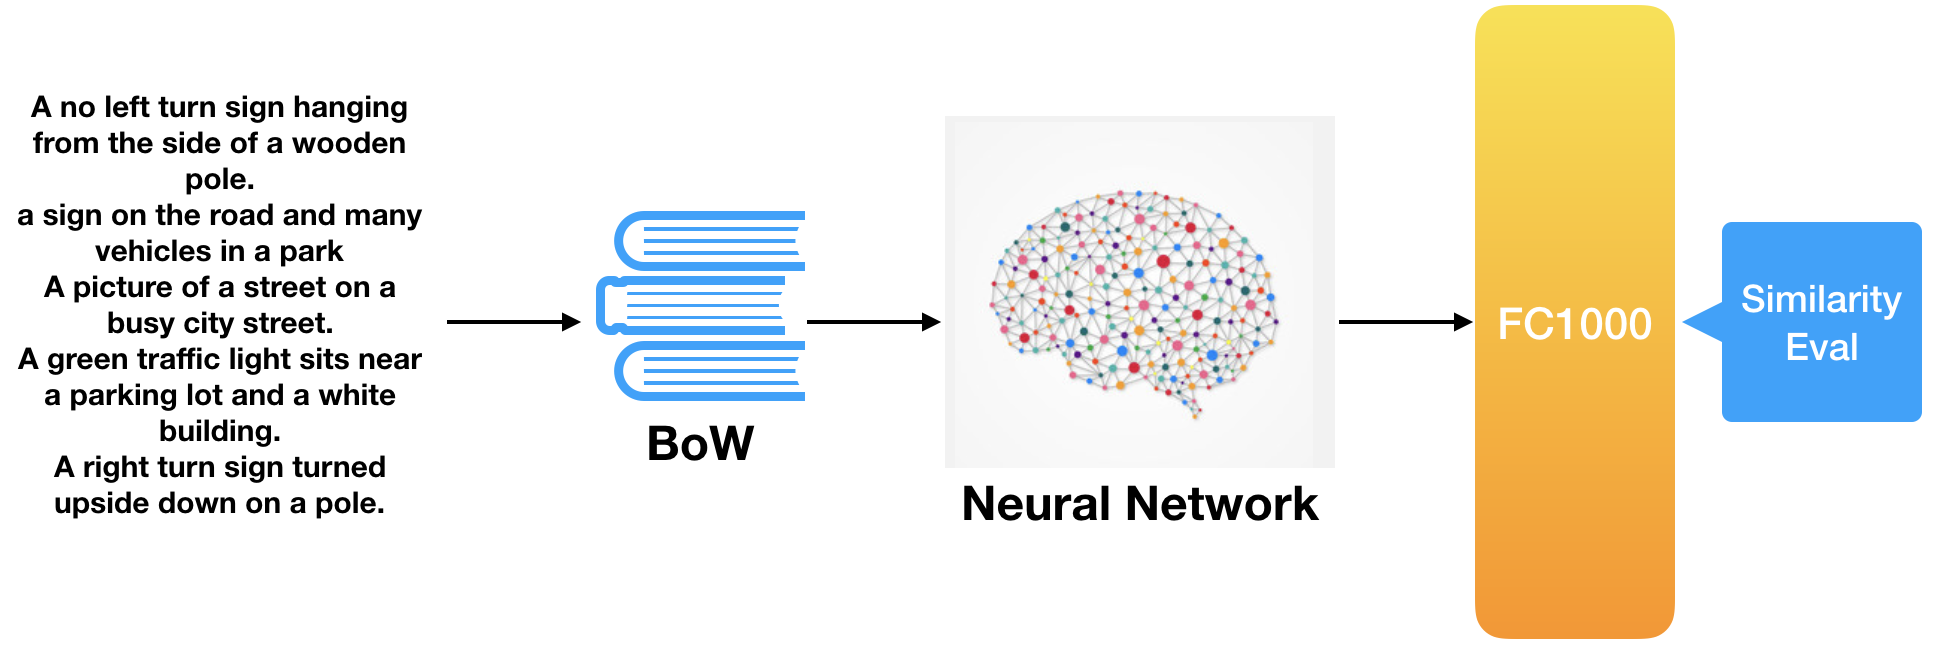
\includegraphics[width=\textwidth]{NNEval}
  \caption{Neural Network Evaluation}
\end{figure}

\subsubsection{PLSR Model}

PLSR models map image feature vectors to BoW representation. In the testing phase, we map the image feature vectors of each image in  the testing set to BoW vectors.

And for each set of descriptions, we first calculation its BoW vector and then compare it with the BoW vectors of the images in testing set based on cosine distance. Then we pick the 20 images with the smallest cosine distance as the result.

\begin{figure}[h]
  \centering
  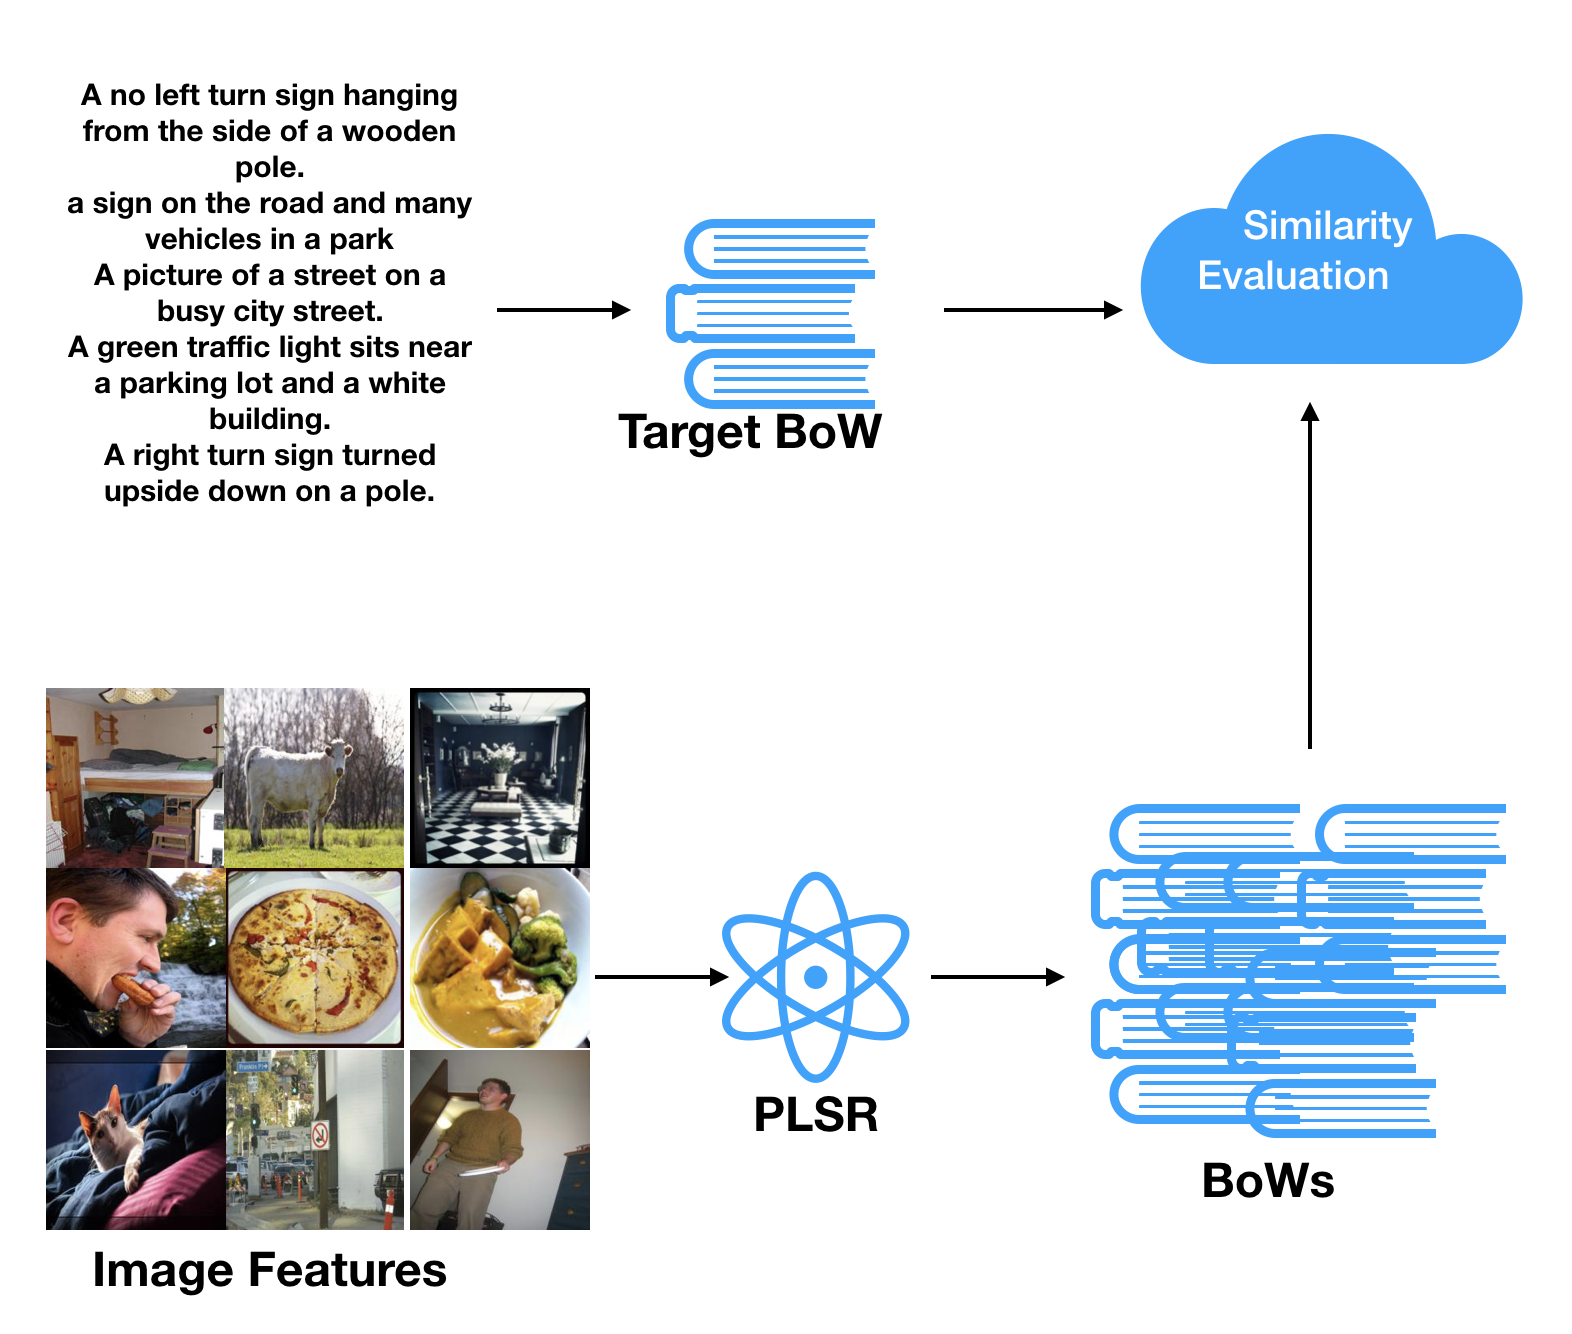
\includegraphics[width=\textwidth]{PLSREval}
  \caption{PLSR Evaluation}
\end{figure}


\subsection{Model Ensemble}

After getting the five models described above (3 PLSR models and 2 Neural Network models), we ensemble them to get a more powerful model. 

The way we get the ensemble model is quite simple: we average the similarity scores from each model and use this averaged score as a new metric to retrieve the 20 images that fit most given a set of descriptions. And finally, we achieve an accuracy score of 0.3695.

\subsection{baihuajun}


\section{Pre-processing the data}
\label{gen_inst}
The training and testing data is downloaded from kaggle website:
\begin{center}
  \url{https://www.kaggle.com/c/cs5785-fall-2017-final/data}
\end{center}
The data has four components in training and testing data, they are images, tags, feature vectors and descriptions. So here we will talk about how we pre-processes each part of data.

\subsection{Pre-processing Description }
n training and test data set, each description points to one image and contains five sentences. The five sentences are similar to each other and contain the same semantic information. We built a dictionary based on the descriptions to make the most of information provided. 
To break down each description, and form a dictionary, we broke sentences into words and throw out the meaningless words in the following steps: \\
(1). Read in each description line by line. \\
(2). Split the descriptions by ”.”, ”,” and ” ” into words. \\
(3). Threw out ”stop words” partially designed by us and partially from Natural Language Toolkit nltk. The so-called ”stop words” are mostly conjunctions, prepositions and numerals which cannot convey solid semantic information.\\
(4). Threw adjectives. We realized that adjectives are harder to predict correctly so that we decided to only use nouns.\\
(5). Extracted all the unique words to put into a dictionary. 
Our dictionary had 3048 words. After having the dictionary, we built bag-of-words for the descrip- tions from training and testing set respectively based on it. 
\subsection{Pre-processing Image Feature Vector and Image Tags }

The first pre-processing step of the image feature vector is sorting. We sorted the feature vector of both of training and testing set, based on image numbers. The pre-process the Image Tag, we used all the tags in the training set to build another dictionary, and build bag-of-words for both of the training and testing tags.



\section{Implement}
\label{headings}

\subsection{BOW+KNN}

While examining the test tags data, we found that some of the tags were phrases instead of words. In the original version, the phrased were stored directly in the dictionary. Since all the descriptions were separated word by word, the phrases wouldn’t be matched at all. Therefore, we split the phrases and stored every single word of tags in the dictionary to achieve a better match. Detailed comparison of accuracy will be discussed in the following chapter Experiments and Results. 
Another aspect of the revision mainly focused on the Bag-of-words representation. During the re- search of previous method, we realized that a weighted BoW representation was better than a binary.

\begin{figure}[h]
  \centering
  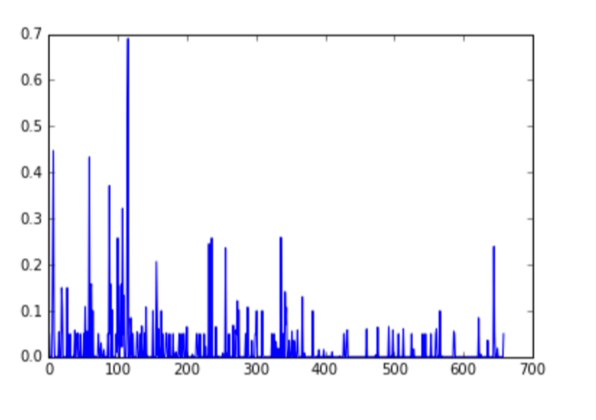
\includegraphics[width=\textwidth]{2}
  \caption{Procedure of Match Tags Method}
\end{figure}
One since words that appeared several times should have more impact on the match of descriptions with tags. We also realized that if a tag appeared in every image, than this tag would be useless in finding the matches. To be more specific, if every image contains an object in common, the matched image would not be found using the tag of that object. To avoid the impact of such common objects, we used a new way of calculating the bag-of-words representation. The BoW representation for each word was the proportion of the times the word appeared in the description or tag file it belonged to the times it appeared in the whole description or tag set.After we trained our BoW representation and predicted the representation of test description. The result is displayed in Figure 3. 

Besides the tags, we map the image in test data with description in training data by using the feature - fc1000. We first use KNN to find 10 nearest features in the training data of each image in testing data and then  do arrogation on all the description of these image. Since we have already prepared the bag of words for all the images in training data, in step, we sum each dimension of the BOW and normalize them. What we get now is a description for each of the image in testing data. Then we do KNN again to find the 20 nearest neighbor of the description and list them in a file.

\subsection{mlx}


\subsection{bhj}


\section{Citations, figures, tables, references}
\label{others}

These instructions apply to everyone.

\subsection{Citations within the text}

The \verb+natbib+ package will be loaded for you by default.
Citations may be author/year or numeric, as long as you maintain
internal consistency.  As to the format of the references themselves,
any style is acceptable as long as it is used consistently.

The documentation for \verb+natbib+ may be found at
\begin{center}
  \url{http://mirrors.ctan.org/macros/latex/contrib/natbib/natnotes.pdf}
\end{center}
Of note is the command \verb+\citet+, which produces citations
appropriate for use in inline text.  For example,
\begin{verbatim}
   \citet{hasselmo} investigated\dots
\end{verbatim}
produces
\begin{quote}
  Hasselmo, et al.\ (1995) investigated\dots
\end{quote}

If you wish to load the \verb+natbib+ package with options, you may
add the following before loading the \verb+nips_2017+ package:
\begin{verbatim}
   \PassOptionsToPackage{options}{natbib}
\end{verbatim}

If \verb+natbib+ clashes with another package you load, you can add
the optional argument \verb+nonatbib+ when loading the style file:
\begin{verbatim}
   \usepackage[nonatbib]{nips_2017}
\end{verbatim}

As submission is double blind, refer to your own published work in the
third person. That is, use ``In the previous work of Jones et
al.\ [4],'' not ``In our previous work [4].'' If you cite your other
papers that are not widely available (e.g., a journal paper under
review), use anonymous author names in the citation, e.g., an author
of the form ``A.\ Anonymous.''

\subsection{Footnotes}

Footnotes should be used sparingly.  If you do require a footnote,
indicate footnotes with a number\footnote{Sample of the first
  footnote.} in the text. Place the footnotes at the bottom of the
page on which they appear.  Precede the footnote with a horizontal
rule of 2~inches (12~picas).

Note that footnotes are properly typeset \emph{after} punctuation
marks.\footnote{As in this example.}

\subsection{Figures}

All artwork must be neat, clean, and legible. Lines should be dark
enough for purposes of reproduction. The figure number and caption
always appear after the figure. Place one line space before the figure
caption and one line space after the figure. The figure caption should
be lower case (except for first word and proper nouns); figures are
numbered consecutively.

You may use color figures.  However, it is best for the figure
captions and the paper body to be legible if the paper is printed in
either black/white or in color.
\begin{figure}[h]
  \centering
  \fbox{\rule[-.5cm]{0cm}{4cm} \rule[-.5cm]{4cm}{0cm}}
  \caption{Sample figure caption.}
\end{figure}

\subsection{Tables}

All tables must be centered, neat, clean and legible.  The table
number and title always appear before the table.  See
Table~\ref{sample-table}.

Place one line space before the table title, one line space after the
table title, and one line space after the table. The table title must
be lower case (except for first word and proper nouns); tables are
numbered consecutively.

Note that publication-quality tables \emph{do not contain vertical
  rules.} We strongly suggest the use of the \verb+booktabs+ package,
which allows for typesetting high-quality, professional tables:
\begin{center}
  \url{https://www.ctan.org/pkg/booktabs}
\end{center}
This package was used to typeset Table~\ref{sample-table}.

\begin{table}[t]
  \caption{Sample table title}
  \label{sample-table}
  \centering
  \begin{tabular}{lll}
    \toprule
    \multicolumn{2}{c}{Part}                   \\
    \cmidrule{1-2}
    Name     & Description     & Size ($\mu$m) \\
    \midrule
    Dendrite & Input terminal  & $\sim$100     \\
    Axon     & Output terminal & $\sim$10      \\
    Soma     & Cell body       & up to $10^6$  \\
    \bottomrule
  \end{tabular}
\end{table}

\section{Final instructions}

Do not change any aspects of the formatting parameters in the style
files.  In particular, do not modify the width or length of the
rectangle the text should fit into, and do not change font sizes
(except perhaps in the \textbf{References} section; see below). Please
note that pages should be numbered.

\section{Preparing PDF files}

Please prepare submission files with paper size ``US Letter,'' and
not, for example, ``A4.''

Fonts were the main cause of problems in the past years. Your PDF file
must only contain Type 1 or Embedded TrueType fonts. Here are a few
instructions to achieve this.

\begin{itemize}

\item You should directly generate PDF files using \verb+pdflatex+.

\item You can check which fonts a PDF files uses.  In Acrobat Reader,
  select the menu Files$>$Document Properties$>$Fonts and select Show
  All Fonts. You can also use the program \verb+pdffonts+ which comes
  with \verb+xpdf+ and is available out-of-the-box on most Linux
  machines.

\item The IEEE has recommendations for generating PDF files whose
  fonts are also acceptable for NIPS. Please see
  \url{http://www.emfield.org/icuwb2010/downloads/IEEE-PDF-SpecV32.pdf}

\item \verb+xfig+ "patterned" shapes are implemented with bitmap
  fonts.  Use "solid" shapes instead.

\item The \verb+\bbold+ package almost always uses bitmap fonts.  You
  should use the equivalent AMS Fonts:
\begin{verbatim}
   \usepackage{amsfonts}
\end{verbatim}
followed by, e.g., \verb+\mathbb{R}+, \verb+\mathbb{N}+, or
\verb+\mathbb{C}+ for $\mathbb{R}$, $\mathbb{N}$ or $\mathbb{C}$.  You
can also use the following workaround for reals, natural and complex:
\begin{verbatim}
   \newcommand{\RR}{I\!\!R} %real numbers
   \newcommand{\Nat}{I\!\!N} %natural numbers
   \newcommand{\CC}{I\!\!\!\!C} %complex numbers
\end{verbatim}
Note that \verb+amsfonts+ is automatically loaded by the
\verb+amssymb+ package.

\end{itemize}

If your file contains type 3 fonts or non embedded TrueType fonts, we
will ask you to fix it.

\subsection{Margins in \LaTeX{}}

Most of the margin problems come from figures positioned by hand using
\verb+\special+ or other commands. We suggest using the command
\verb+\includegraphics+ from the \verb+graphicx+ package. Always
specify the figure width as a multiple of the line width as in the
example below:
\begin{verbatim}
   \usepackage[pdftex]{graphicx} ...
   \includegraphics[width=0.8\linewidth]{myfile.pdf}
\end{verbatim}
See Section 4.4 in the graphics bundle documentation
(\url{http://mirrors.ctan.org/macros/latex/required/graphics/grfguide.pdf})

A number of width problems arise when \LaTeX{} cannot properly
hyphenate a line. Please give LaTeX hyphenation hints using the
\verb+\-+ command when necessary.

\subsubsection*{Acknowledgments}

Use unnumbered third level headings for the acknowledgments. All
acknowledgments go at the end of the paper. Do not include
acknowledgments in the anonymized submission, only in the final paper.

\section*{References}

References follow the acknowledgments. Use unnumbered first-level
heading for the references. Any choice of citation style is acceptable
as long as you are consistent. It is permissible to reduce the font
size to \verb+small+ (9 point) when listing the references. {\bf
  Remember that you can go over 8 pages as long as the subsequent ones contain
  \emph{only} cited references.}
\medskip

\small

[1] Alexander, J.A.\ \& Mozer, M.C.\ (1995) Template-based algorithms
for connectionist rule extraction. In G.\ Tesauro, D.S.\ Touretzky and
T.K.\ Leen (eds.), {\it Advances in Neural Information Processing
  Systems 7}, pp.\ 609--616. Cambridge, MA: MIT Press.

[2] Bower, J.M.\ \& Beeman, D.\ (1995) {\it The Book of GENESIS:
  Exploring Realistic Neural Models with the GEneral NEural SImulation
  System.}  New York: TELOS/Springer--Verlag.

[3] Hasselmo, M.E., Schnell, E.\ \& Barkai, E.\ (1995) Dynamics of
learning and recall at excitatory recurrent synapses and cholinergic
modulation in rat hippocampal region CA3. {\it Journal of
  Neuroscience} {\bf 15}(7):5249-5262.

\end{document}